\section{snode Strukturreferenz}
\label{structsnode}\index{snode@{snode}}
{\tt \#include $<$hashtab.h$>$}

Zusammengeh\"{o}rigkeiten von snode:\begin{figure}[H]
\begin{center}
\leavevmode
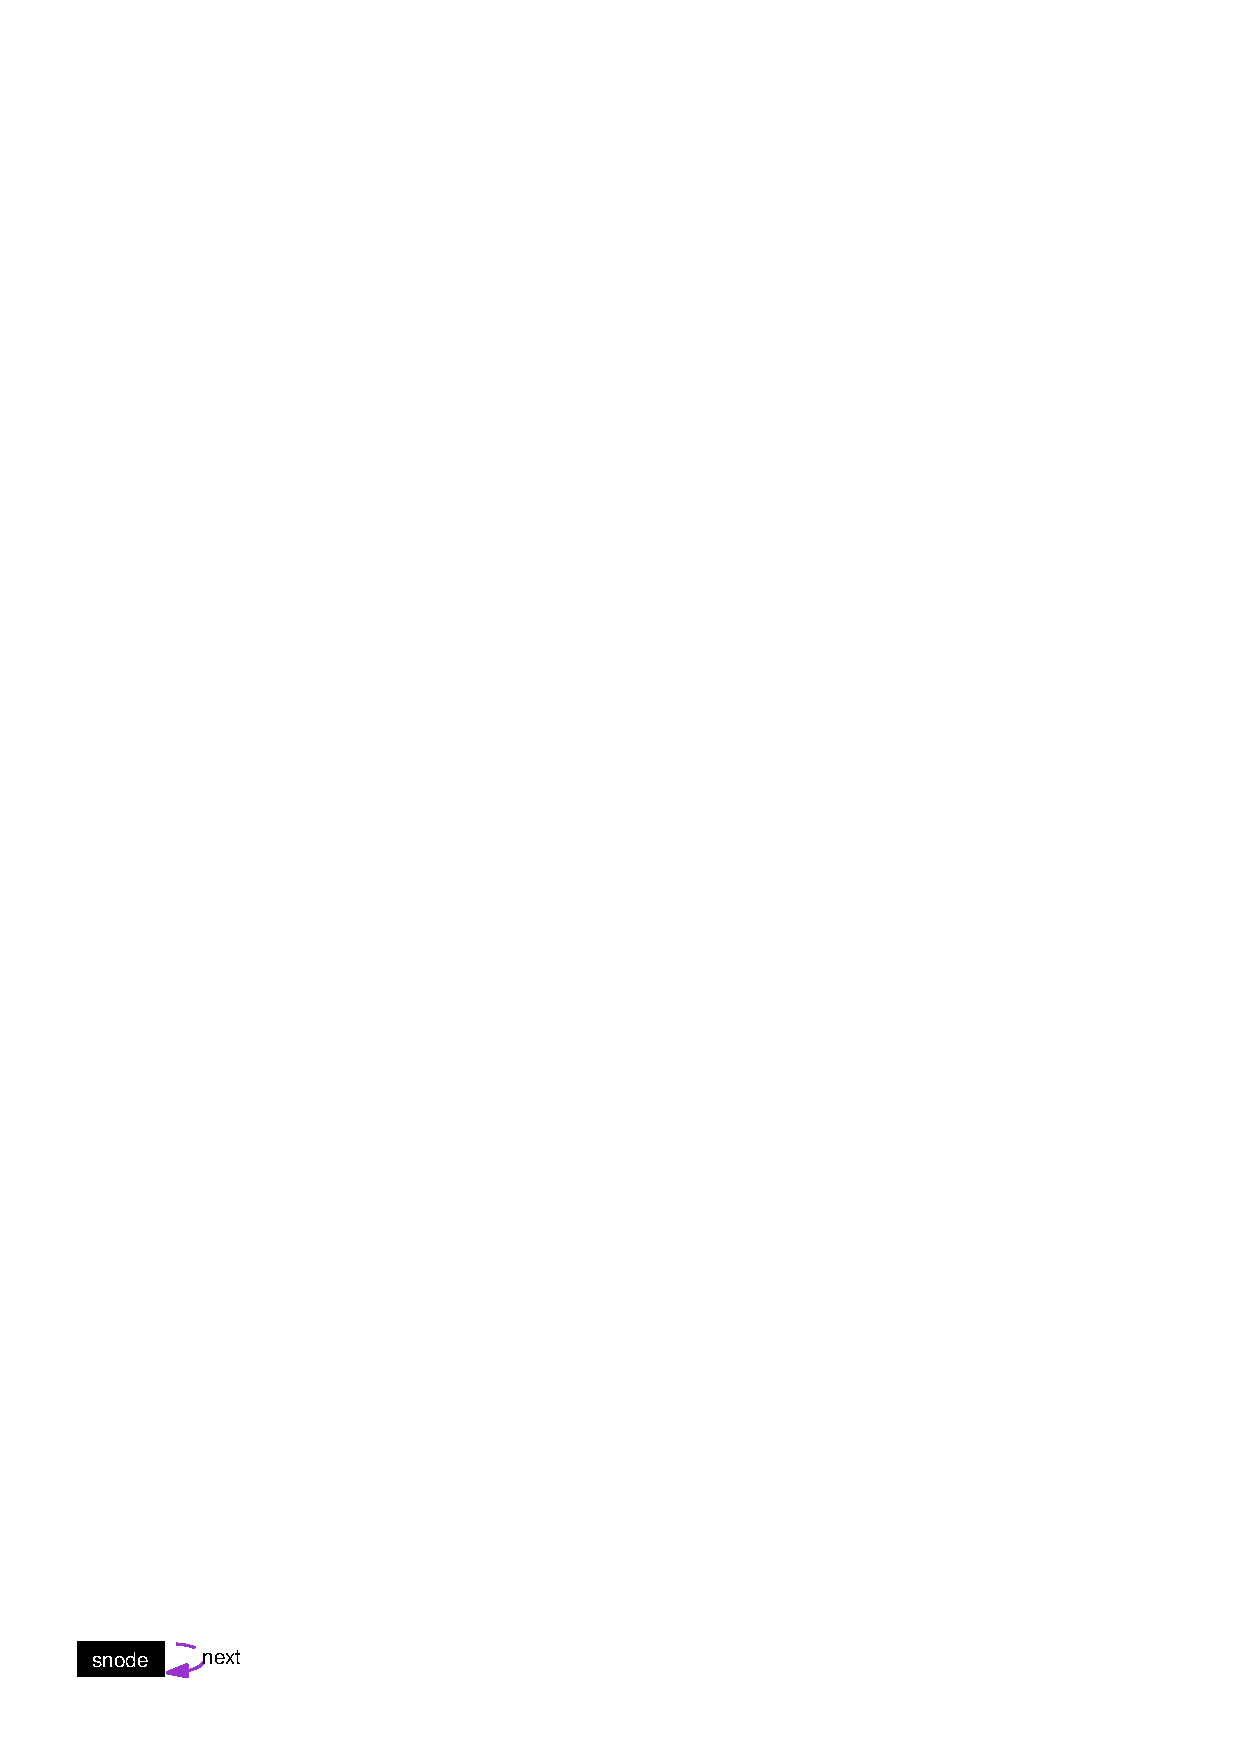
\includegraphics[width=59pt]{structsnode__coll__graph}
\end{center}
\end{figure}
\subsection*{Datenfelder}
\begin{CompactItemize}
\item 
char $\ast$ {\bf string}
\item 
u\_\-long {\bf count}
\item 
{\bf snode} $\ast$ {\bf next}
\end{CompactItemize}


\subsection{Ausf\"{u}hrliche Beschreibung}




Definiert in Zeile 55 der Datei hashtab.h.

\subsection{Dokumentation der Datenelemente}
\index{snode@{snode}!count@{count}}
\index{count@{count}!snode@{snode}}
\subsubsection{\setlength{\rightskip}{0pt plus 5cm}u\_\-long {\bf snode::count}}\label{structsnode_af14980bcdb9d5e9543507adee3fd803}




Definiert in Zeile 56 der Datei hashtab.h.

Wird benutzt von all\_\-search\_\-page(), dump\_\-all\_\-search(), new\_\-snode(), put\_\-snode() und top\_\-search\_\-table().\index{snode@{snode}!next@{next}}
\index{next@{next}!snode@{snode}}
\subsubsection{\setlength{\rightskip}{0pt plus 5cm}struct {\bf snode}$\ast$ {\bf snode::next}}\label{structsnode_91a76319ab431b979edd96540899a605}




Definiert in Zeile 57 der Datei hashtab.h.

Wird benutzt von del\_\-slist(), load\_\-srch\_\-array() und put\_\-snode().\index{snode@{snode}!string@{string}}
\index{string@{string}!snode@{snode}}
\subsubsection{\setlength{\rightskip}{0pt plus 5cm}char$\ast$ {\bf snode::string}}\label{structsnode_4917005c761d2dfdb653d88a2eb5aa58}




Definiert in Zeile 55 der Datei hashtab.h.

Wird benutzt von all\_\-search\_\-page(), del\_\-slist(), dump\_\-all\_\-search(), new\_\-snode(), put\_\-snode() und top\_\-search\_\-table().

Die Dokumentation f\"{u}r diese Struktur wurde erzeugt aufgrund der Datei:\begin{CompactItemize}
\item 
oosalizer/{\bf hashtab.h}\end{CompactItemize}
